\documentclass[notes,11pt, aspectratio=169]{beamer}


\usepackage{pgfpages}
% These slides also contain speaker notes. You can print just the slides,
% just the notes, or both, depending on the setting below. Comment out the want
% you want.
\setbeameroption{hide notes} % Only slide
%\setbeameroption{show only notes} % Only notes
%\setbeameroption{show notes on second screen=right} % Both

\usepackage{helvet}
\usepackage[default]{lato}
\usepackage{array}
\usepackage{tgbonum}


\usepackage{txfonts} % https://www.ctan.org/tex-archive/fonts/txfonts

\usepackage{tikz}
\usepackage{verbatim}
\setbeamertemplate{note page}{\pagecolor{yellow!5}\insertnote}
\usetikzlibrary{positioning}
\usetikzlibrary{snakes}
\usetikzlibrary{calc}
\usetikzlibrary{arrows}
\usetikzlibrary{decorations.markings}
\usetikzlibrary{shapes.misc}
\usetikzlibrary{matrix,shapes,arrows,fit,tikzmark}
\usepackage{amsmath}
\usepackage{mathpazo}
\usepackage{hyperref}
\usepackage{lipsum}
\usepackage{multimedia}
\usepackage{graphicx}
\usepackage{multirow}
\usepackage{dcolumn}
\usepackage{bbm}
\newcolumntype{d}[0]{D{.}{.}{5}}

\usepackage{changepage}
\usepackage{appendixnumberbeamer}
\newcommand{\beginbackup}{
   \newcounter{framenumbervorappendix}
   \setcounter{framenumbervorappendix}{\value{framenumber}}
   \setbeamertemplate{footline}
   {
     \leavevmode%
     \hline
     box{%
       \begin{beamercolorbox}[wd=\paperwidth,ht=2.25ex,dp=1ex,right]{footlinecolor}%
%         \insertframenumber  \hspace*{2ex} 
       \end{beamercolorbox}}%
     \vskip0pt%
   }
 }
\newcommand{\backupend}{
   \addtocounter{framenumbervorappendix}{-\value{framenumber}}
   \addtocounter{framenumber}{\value{framenumbervorappendix}} 
}


\usepackage{graphicx}
\usepackage[space]{grffile}
\usepackage{booktabs}
\newcommand\independent{\protect\mathpalette{\protect\independenT}{\perp}}
\def\independenT#1#2{\mathrel{\rlap{$#1#2$}\mkern2mu{#1#2}}}
\DeclareMathOperator{\Supp}{Supp}
% so that the captions are numerated
\setbeamertemplate{caption}[numbered]





% These are my colors -- there are many like them, but these ones are mine.
\definecolor{blue}{RGB}{0,114,178}
\definecolor{red}{RGB}{213,94,0}
\definecolor{yellow}{RGB}{240,228,66}
\definecolor{green}{RGB}{0,158,115}
\definecolor{jet}{HTML}{131516}

\hypersetup{
  colorlinks=false,
  linkbordercolor = {white},
  linkcolor = {blue}
}


%% I use a beige off white for my background
\definecolor{MyBackground}{RGB}{255,253,218}

%% Uncomment this if you want to change the background color to something else
%\setbeamercolor{background canvas}{bg=MyBackground}

%% Change the bg color to adjust your transition slide background color!
\newenvironment{transitionframe}{
  \setbeamercolor{background canvas}{bg=white}
  \begin{frame}}{
    \end{frame}
}


\setbeamercolor{frametitle}{fg=blue}
\setbeamercolor{title}{fg=black}
\setbeamertemplate{footline}[frame number]
\setbeamertemplate{navigation symbols}{} 
\setbeamertemplate{itemize items}{$\blacktriangleright$}
\setbeamercolor{itemize item}{fg=blue}
\setbeamercolor{itemize subitem}{fg=blue}
\setbeamercolor{enumerate item}{fg=blue}
\setbeamercolor{enumerate subitem}{fg=blue}
\setbeamercolor{button}{bg=MyBackground,fg=blue,}
% Block
\setbeamercolor{block title}{fg = white, bg =blue}
\setbeamercolor{block body}{fg = jet, bg = jet!10!white}


% If you like road maps, rather than having clutter at the top, have a roadmap show up at the end of each section 
% (and after your introduction)
% Uncomment this is if you want the roadmap!
% \AtBeginSection[]
% {
%    \begin{frame}
%        \frametitle{Roadmap of Talk}
%        \tableofcontents[currentsection]
%    \end{frame}
% }
\setbeamercolor{section in toc}{fg=blue}
\setbeamercolor{subsection in toc}{fg=red}
\setbeamersize{text margin left=1em,text margin right=1em} 

\newenvironment{wideitemize}{\itemize\addtolength{\itemsep}{10pt}}{\enditemize}

\usepackage{environ}
\NewEnviron{videoframe}[1]{
  \begin{frame}
    \vspace{-8pt}
    \begin{columns}[onlytextwidth, T] % align columns
      \begin{column}{.70\textwidth}
        \begin{minipage}[t][\textheight][t]
          {\dimexpr\textwidth}
          \vspace{8pt}
          \hspace{4pt} {\Large \sc \textcolor{blue}{#1}}
          \vspace{8pt}
          
          \BODY
        \end{minipage}
      \end{column}%
      \hfill%
      \begin{column}{.38\textwidth}
        \colorbox{green!20}{\begin{minipage}[t][1.2\textheight][t]
            {\dimexpr\textwidth}
            Face goes here
          \end{minipage}}
      \end{column}%
    \end{columns}
  \end{frame}
}

%%% TIKZ STUFF
\tikzset{   
        every picture/.style={remember picture,baseline},
        every node/.style={anchor=base,align=center,outer sep=1.5pt},
        every path/.style={thick},
        }
\newcommand\marktopleft[1]{%
    \tikz[overlay,remember picture] 
        \node (marker-#1-a) at (-.3em,.3em) {};%
}
\newcommand\markbottomright[2]{%
    \tikz[overlay,remember picture] 
        \node (marker-#1-b) at (0em,0em) {};%
}
\tikzstyle{every picture}+=[remember picture] 
\tikzstyle{mybox} =[draw=black, very thick, rectangle, inner sep=10pt, inner ysep=20pt]
\tikzstyle{fancytitle} =[draw=black,fill=red, text=white]
%%%% END TIKZ STUFF



%title
\title{\textcolor{blue}{Identification and Estimation of Treatment and Interference Effects in Observational Studies on Networks}\footnote{\href{https://www.tandfonline.com/doi/full/10.1080/01621459.2020.1768100?scroll=top&needAccess=true}{\textcolor{blue}{Source : }}Forastiere L, Airoldi E M, Mealli F. Identification and estimation of treatment and interference effects in observational studies on networks[J]. Journal of the American Statistical Association, 2021, 116(534): 901-918.}}
\author{}
\institute{\small{Nankai University}}
\date{\today}


\begin{document}

% Title Slide
\begin{frame}
\maketitle

\end{frame}


% INTRO
\begin{frame}{Interference}
\begin{columns}[T] % align columns
\begin{column}{\textwidth}
  \begin{wideitemize}
  \item  Interference is said to be present when a treatment, exposure, or intervention, on one unit has an effect on the response of another unit [\href{https://philpapers.org/rec/COXPOE}{\textcolor{blue}{Cox 1958}}]  
  \begin{figure}[h]
      \centering
      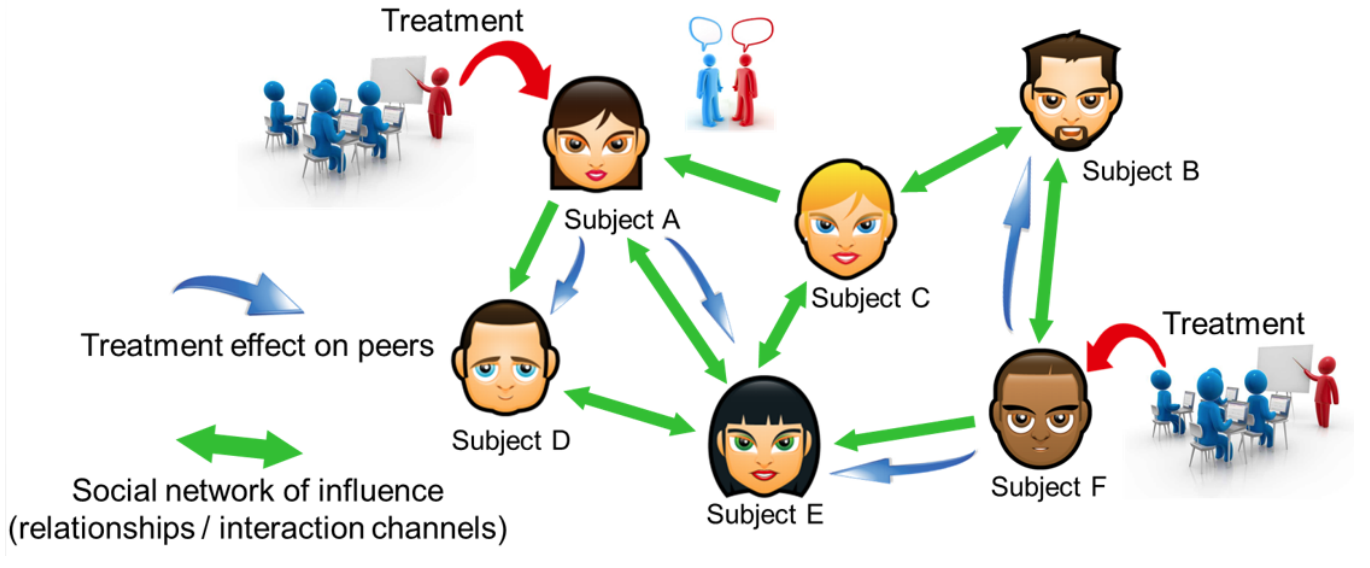
\includegraphics[scale=0.45]{figure1.png}
      \caption{from \href{https://arxiv.org/abs/1708.08522}{\textcolor{red}{Kao(2017)}}}
      \label{fig:fig1}
  \end{figure}
  \end{wideitemize}
\end{column}%
\end{columns}
\end{frame}
%   \makebox[\linewidth][c]{
%     \resizebox{\linewidth}{!}{
% %      \includegraphics{how-to-draw-an-owl.pdf}
%     }}

% INTRO
\begin{frame}{Interference effect in causal inference}
\begin{columns}[T] % align columns
\begin{column}{0.95\textwidth}
  \begin{wideitemize}
  \item assume no interference effect  [contained in SUTVA,Rubin \href{https://www.jstor.org/stable/2287653}{\textcolor{blue}{ 1980}}] ,   \item unreasonable and risky (Sobel \href{https://www.tandfonline.com/doi/abs/10.1198/016214506000000636}{\textcolor{blue}{2006}})
  \item Experimental studies : 
  \begin{itemize}
  \vspace{10pt}
      \item cluster randomized trials , two stage randomization (Hudgens and Halloran \href{https://www.ncbi.nlm.nih.gov/pmc/articles/PMC2600548/}{\textcolor{blue}{2008}}; Sinclair \href{https://www.cambridge.org/core/books/abs/cambridge-handbook-of-experimental-political-science/design-and-analysis-of-experiments-in-multilevel-populations/5A74D87743BB688894BB8002A837C402}{\textcolor{blue}{2011}}) , Insulated Neighbors Randomization (Toulis and Kao \href{https://proceedings.mlr.press/v28/toulis13.html}{\textcolor{blue}{2013}}) 
      \vspace{10pt}
      \item test and estimate the total treatment effect ( Rosenbaum \href{https://www.tandfonline.com/doi/abs/10.1198/016214506000001112?journalCode=uasa20}{\textcolor{blue}{2007}}), separately test for treatment and spillover effects (Bowers, Fredrickson, and Panagopoulos \href{https://www.cambridge.org/core/journals/political-analysis/article/abs/reasoning-about-interference-between-units-a-general-framework/0E2410C1A5666EE5ACA4CBE29AFFFAE7}{\textcolor{blue}{2013}}) ,  Horvitz–Thompson estimator (Aronow and Samii \href{https://arxiv.org/abs/1305.6156}{\textcolor{blue}{2017}})
  \end{itemize} 
  \end{wideitemize}
\end{column}%
\hfill%
\begin{column}{.38\textwidth}
\end{column}%
\end{columns}
\end{frame}



\begin{frame}{Interference effect in causal inference}
\begin{columns}[T] % align columns
\begin{column}{0.95\textwidth}
  \begin{wideitemize}
  \item spillover effect for observational studies 
  \begin{itemize}
      \item parametric multilevel approach (Raudenbush \href{https://www.tandfonline.com/doi/abs/10.1198/016214506000000447}{\textcolor{blue}{2006}}) , three-level generalized hierarchical linear model (Verbitsky-Savitz and Raudenbush \href{https://www.degruyter.com/document/doi/10.1515/2161-962X.1020/html?lang=en}{\textcolor{blue}{2012}}) , IPW estimators (Tchetgen Tchetgen and VanderWeele \href{https://www.ncbi.nlm.nih.gov/pmc/articles/PMC4216807/}{\textcolor{blue}{2012}})
  \end{itemize} 
  \item causal inference for observational studies
  \begin{itemize}
     \item generalized IPW estimator  (Liu et al. \href{https://www.ncbi.nlm.nih.gov/pmc/articles/PMC5793685/}{\textcolor{blue}{2016}}) , targeted maximum likelihood estimator (TMLE) (Sofrygin and van der Laan  \href{https://www.ncbi.nlm.nih.gov/pmc/articles/PMC5650205/}{\textcolor{blue}{2017}}) , extended this TMLE estimator to allow for dependence (Ogburn et al \href{https://arxiv.org/abs/1705.08527}{\textcolor{blue}{2017}})
  \end{itemize}
  \end{wideitemize}
\end{column}%
\hfill%
\begin{column}{.38\textwidth}

\end{column}%
\end{columns}
\end{frame}













\begin{frame}{Contents}
\begin{columns}[T] % align columns
\begin{column}{.8\textwidth}
  \begin{enumerate}[{Part} I.]
    \item Causal problem and identification
    \item Bias analysis
    \item Proposed method
    \item Simulation studies
    \item Conclusion
  \end{enumerate}
\end{column}
\end{columns}
\end{frame}



\section{Causal problem and identification}
\begin{transitionframe}
  \begin{center}
    { \Huge \textcolor{blue}{I. Causal problem and identification}}
  \end{center}
\end{transitionframe}






\begin{frame}{Notation}
\begin{columns}[T] % align columns
\begin{column}{.8\textwidth}
  \begin{wideitemize}
  %
  \item  Undirected network $G=(\mathcal{N},\mathbb{E})$
  \item  Treatment $Z_i \in \left\{0,1\right\}$,  outcome $Y_i \in \mathcal{Y}$
  \item  covariates $ \mathbf{X}_i \in \mathcal{X}$ ,individual covariates $\mathbf{X}_{i}^{ind} \in \mathcal{X}^{ind}$,neighborhood covariates $\mathbf{X}_{i}^{neigh} \in \mathcal{X}^{neigh}$
  \item  For unit i, consider partition $(i,\mathcal{N}_i,\mathcal{N}_{-i})$ , $(Z_i , \mathbf{Z}_{\mathcal{N}_i},\mathbf{Z}_{\mathcal{N}_{-i}})$ , $(Y_i , \mathbf{Y}_{\mathcal{N}_i},\mathbf{Y}_{\mathcal{N}_{-i}})$ 
  %
  \end{wideitemize}
\end{column}%
\hfill%
\begin{column}{.38\textwidth}
\end{column}%
\end{columns}
\end{frame}

\begin{frame}{Potential Outcomes and Neighborhood Interference}
\begin{itemize}
    \item \textbf{\emph{Stable unit treatment on neighborhood value assumption (SUTNVA)}}
\end{itemize}
%
\begin{block}{Assumption 1 (No multiple version of   treatment(consistency))}\label{assump1}
\centering
If \ $\mathbf{Z}$=$\mathbf{z}$ \  then \  $Y_i=Y_i(\mathbf{z})$  
\end{block}
  \\
\begin{block}{Assumption 2 (Neighborhood interference)}\label{assump2}
Given a function $g_i \colon \left\{0,1\right\}^{\mathcal{N}_i} \rightarrow \mathcal{G}_i$,$\forall i \in \mathcal{N}$  , $\forall \mathbf{Z}_{\mathcal{N}_{-i}}$ , $\mathbf{Z}'_{\mathcal{N}_{-i}}$ and $\forall  \mathbf{Z}_{\mathcal{N}_{i}}$ , $\mathbf{Z}'_{\mathcal{N}_{i}}$ : $g_i(\mathbf{Z}_{\mathcal{N}_i})=g_i(\mathbf{Z}'_{\mathcal{N}_i})$ , the following equality holds :
    \\
\centering
    $Y_i(Z_i,\mathbf{Z}_{\mathcal{N}_i},\mathbf{Z}_{\mathcal{N}_{-i}})=Y_i(Z_i,\mathbf{Z}'_{\mathcal{N}_i},\mathbf{Z}'_{\mathcal{N}_{-i}})$
\end{block}
%
Each unit's potential outcome is subject to two treatments : the \emph{individual treatment }$Z_i$ , and \emph{the neighborhood treatment} $G_i$ [$G_i=g_i(\mathbf{Z}_{\mathcal{N}_i}) \in \mathcal{G}_i$]
%
\end{frame}


\begin{frame}{Individual and Neighborhood Treatments}	
%
\begin{itemize}
    \item The assignment mechanism is the \textbf{\emph{probability distribution of the joint treatment}} in the whole sample, given all covariates and potential outcomes.
\end{itemize}
%
\vspace{1em}
\centering
\begin{equation*}
P(\mathbf{Z},\mathbf{G}|\mathbf{X},\{\mathbf{Y}(z,g),z=0,1;g \in \mathcal{G}\})=
\\
\left\{\begin{array}{ccc}P(\mathbf{Z}|\mathbf{X},\left\{\mathbf{Y}(z,g),z=0,1;g \in \mathcal{G} \right\}) & \mbox{if} & \mathbf{G}=\mathbf{g}(\mathbf{Z}) \\ 0 &  & otherwise \end{array}\right.  
\end{equation*}
%
\end{frame}


\begin{frame}{Causal Estimands : Main Effects and Spillover effects}
\begin{block}{Average dose-response function
(ADRF)}
\centering
$\mu(z,g;V)=E[Y_i(z,g)|i \in V]$ \qquad $\forall z \in \{0,1\}, g \in \mathcal{G}$
\end{block}  
%
\begin{block}{Main effect $\tau(g)$ and overall main effect $\tau$}
\centering
$\tau(g)=\mu(1,g;V_g)-\mu(0,g;V_g)$
\\
\centering
$\tau=\sum_{g \in \mathcal{G}} \tau(g)P(G_i=g)$
\end{block}  
%
\begin{block}{Spillover effect $\delta(g;z)$ and overall spillover effect $\Delta(z)$}
\centering
$\delta(g;z)=\mu(z,g;V_g)-\mu(z,0;V_g)$
\\
\centering
$\Delta(z)=\sum_{g \in \mathcal{G}} \delta(g;z)P(G_i=g)$
\end{block}  
%
\centering
$ TE= \sum_{g \in \mathcal{G}}E[Y_i(Z_i=1,G_i=g)-Y_i(Z_i=0,G_i=0)| i \in V_g]P(G_i=g)=\tau +\Delta(0)
$
\end{frame}




\begin{frame}{Unconfoundedness of the Joint Treatment}
\begin{block}{Assumption 3 (Unconfoundedness of individual and neighborhood treatment)}\label{assump3}
\centering
$Y_i(z,g) \perp\!\!\!\perp Z_i,G_i|\mathbf{X}_i$ \qquad $\forall z \in \{0,1\} , g \in \mathcal{G}_i , \forall i$
\end{block}
\vspace{1em}
%
\begin{block}{Theorem 1 (Identification of ADRF)}
Under  \hyperlink{assump1}{\textcolor{blue}{Assumption 1}} (no multiple versions of treatment), \hyperlink{assump2}{\textcolor{blue}{Assumption2}} (neighborhoood interference) , and \hyperlink{assump3}{\textcolor{blue}{Assumption 3}} (unconfoundedness) , we have 
\\
\centering
$E[Y_i(z,g)|i \in V_g]= \sum_{\mathbf{x} \in \mathcal{X}}E[Y_i|Z_i=z,G_i=g,\mathbf{X_i}=\mathbf{x}, i \in V_g]P(\mathbf{X_i}=\mathbf{x} | i \in V_g) $
\end{block}
\end{frame}



\section{Bias analysis}
\begin{transitionframe}
  \begin{center}
    { \Huge \textcolor{blue}{II. Bias analysis}}
  \end{center}
\end{transitionframe}


\begin{frame}{Bias When SUTVA Is Wrongly Assumed}
Under SUTVA ,average (individual) treatment effect : $\tau_{sutva}=E[Y_i(Z_i=1)-Y_i(Z_i=0)]$
\vspace{1em}
\begin{block}{Naive estimator}
\centering
$\tau_{\mathbf{X}^\star}^{obs}=\sum_{\mathbf{x} \in \mathcal{X}^\star}(E[Y_i|Z_i=1,\mathbf{X}_{i}^\star]-E[Y_i|Z_i=1,\mathbf{X}_{i}^\star])P(\mathbf{X}_{i}^\star=\mathbf{x})$
\end{block}
%
\vspace{1em}
The difference between $\tau$  and the quantity $\tau_{\mathbf{X}^\star}^{obs}$ represents the bias for $\tau$ of a naive approach that neglects interference
\end{frame}

\begin{frame}{Bias of Naive Estimator When Unconfoudedness Holds}
\begin{block}{Theorem 2.A} \label{theorem 2.A}
Let $G=(\mathcal{N},\mathbb{E}$ be a known social network and lei $\mathcal{N}_i$ be the neighborhood of unit i asa defined by the presence of edges . Let $Z_i \in \{0,1\}$ be a binary treatment assigned to unit i and let $G_i$ be a deterministic function of the subset of the treatment vector $\mathbf{Z}$ in the neighborhood $\mathcal{N}_i$ , that is , $ G_i = g_i(\mathbf{Z}_{\mathcal{N}_i})$ , with $g_i : \{0,1\}^{N_i} \rightarrow \mathcal{G}_i$ . If
\begin{enumerate}
    \item \hyperlink{assump1}{\textcolor{blue}{Assumption 1}} holds
    \item \hyperlink{assump2}{\textcolor{blue}{Assumption 2}} holds , given function $g_i(\cdot)$ for each unit $i \in \mathcal{N}$
    \item \hyperlink{assump3}{\textcolor{blue}{Assumption 3}} holds conditional on $\mathbf{X}_{i}^\star$ , that is , $Y_i(z,g) \perp\!\!\!\perp Z_i,G_i|\mathbf{X}_{i}^\star$, $\forall z \in \{0,1\} , g \in \mathcal{G}_i$
\end{enumerate}
then the following equality holds
\begin{align*}
\tau_{\mathbf{X}^\star}^{obs}&=\sum_{\mathbf{x} \in \mathcal{X}^\star} \Big( \sum_{g \in \mathcal{G}}E[Y_i(1,g)|\mathbf{X}_{i}^\star = \mathbf{x}, i \in V_g]P(G_i=g | Z_i=1 , \mathb , i \in \matf{X}_{i}^\star=\mathbf{x}) 
\\  &  -E[Y_i(0,g)|,\mathbf{X}_{i}^\star =\mathbf{x} , i \in V_g]P(G_i=g | Z_i=0,\mathbf{X}_{i}^\star=\mathbf{x})  \Big)  P(\mathbf{X}_{i}^\star=\mathbf{x}) %
\end{align*}
\end{block}
\end{frame}



\begin{frame}{Bias of Naive Estimator When Unconfoudedness Holds}
\begin{block}{Corollary 1}
Under the three conditions of \hyperlink{theorem2.A}{\textcolor{blue}{Theorem 2.A}} and the additional condition
\begin{enumerate}
    \item[4.] $Z_i$ and $G_i$ are independent conditional on $\mathbf{X}_{i}^\star$ , that is , $Z_i \perp\!\!\!\perp G_i |\mathbf{X}_{i}^\star$
\end{enumerate}
%
the following equality holds :
\begin{equation*}
    \tau_{\mathbf{X}^\star}^{obs}=\tau
\end{equation*}
%
\end{block}
\begin{block}{Corollary 2}
Under the three conditions of \hyperlink{theorem2.A}{\textcolor{blue}{Theorem 2.A}} and $Z_i \not \! \perp\!\!\!\perp G_i |\mathbf{X}_{i}^\star$ , an unbiased estimator of $\tau_{\mathbf{X}^\star}^{obs}$ would be biased for the overall main effect $\tau$ , with bisas given by
%
\end{block}
\end{frame}


\begin{frame}{Bias of Naive Estimator When Unconfoudedness Holds}
\begin{block}{Corollary 2 continued}
\begin{align*}
   \tau_{\mathbf{X}^\star}^{obs}-\tau &=\sum_{\mathbf{x} \in \mathcal{X}^\star}  \sum_{g \in \mathcal{G}} \Big( E[Y_i|Z_i=1 , G_i=g , \mathbf{X}_{i}^\star =\mathbf{x}, i \in V_g]
\\ &   -E[Y_i|Z_i=1,G_i=g' , \mathbf{X}_{i}^\star =\mathbf{x} , i \in V_g]\Big)
\\ & \Big(P(G_i=g | Z_i=1,\mathbf{X}_{i}^\star=\mathbf{x}) - P(G_i=g | \mathbf{X}_{i}^\star=\mathbf{x})   \Big)  P(\mathbf{X}_{i}^\star=\mathbf{x})
\\ & - \sum_{\mathbf{x} \in \mathcal{X}^\star}  \sum_{g \in \mathcal{G}} \Big(E[Y_i|Z_i=0 , G_i=g , \mathbf{X}_{i}^\star =\mathbf{x}, i \in V_g]
\\  &  -E[Y_i|Z_i=0,G_i=g' , \mathbf{X}_{i}^\star =\mathbf{x} , i \in V_g]\Big)
\\ & \Big(P(G_i=g | Z_i=0,\mathbf{X}_{i}^\star=\mathbf{x}) - P(G_i=g | \mathbf{X}_{i}^\star=\mathbf{x})   \Big)  P(\mathbf{X}_{i}^\star=\mathbf{x})
\end{align*}
\end{block}
\end{frame}


\begin{frame}{Bias of Naive Estimator When Unconfoudedness Does Not Hold}
\begin{block}{Theorem 2.B} \label{theorem2.B}
Under \hyperlink{assump1}{\textcolor{blue}{Assumption 1}} and \hyperlink{assump2}{\textcolor{blue}{2}} , if  \hyperlink{assump3}{\textcolor{blue}{Assumption 3}} does not hold conditional on $\mathbf{X}_{i}^\star$ ,that is $Y_i(z,g) \not \! \perp\!\!\!\perp Z_i,G_i|\mathbf{X}_{i}^\star$ , but holds conditioanl on $\mathbf{X}_{i}^\star$ and an additional vector of covariates $\mathbf{U}_i \in \mathcal{U}$ , that is , $Y_i(z,g) \perp\!\!\!\perp Z_i,G_i|\mathbf{X}_{i}^\star , \mathbf{U}_i$ , an unbiased estimator of $\tau_{\mathbf{X}^\star}^{obs}$ would be unbiased for the overall main effect $\tau$ , with bias $\tau_{\mathbf{X}^\star}^{obs} - \tau$ given by
%
\begin{align*}
&=\sum_{\mathbf{x} \in \mathcal{X}^\star}  \sum_{g \in \mathcal{G}} \sum_{u \in \mathcal{U}} \Big( E[Y_i|Z_i=1 , G_i =g , \mathbf{U}_i = \mathbf{u} , \mathbf{X}_{i}^\star = \mathbf{x}, i \in V_g] 
\\ & - E[Y_i|Z_i=1 , G_i =g' , \mathbf{U}_i = \mathbf{u}' , \mathbf{X}_{i}^\star = \mathbf{x}, i \in V_g] \Big)
\\ & \Big( P( \mathbf{U}_i = \mathbf{u} |, Z_i=1 , G_i =g , \mathbf{X}_{i}^\star = \mathbf{x})P( G_i =g | Z_i=1 ,  \mathbf{X}_{i}^\star = \mathbf{x})
\\ & - P( \mathbf{U}_i = \mathbf{u} | G_i =g , \mathbf{X}_{i}^\star = \mathbf{x})P( G_i =g | \mathbf{X}_{i}^\star = \mathbf{x}) \Big) P(\mathbf{X}_{i}^\star = \mathbf{x})
%
\end{align*}
\end{block}
\end{frame}


\begin{frame}{Bias of Naive Estimator When Unconfoudedness Does Not Hold}
\begin{block}{Theorem 2.B continued}
%
\begin{align*}
    & = \sum_{\mathbf{x} \in \mathcal{X}^\star}  \sum_{g \in \mathcal{G}} \sum_{u \in \mathcal{U}} \Big( E[Y_i|Z_i=0 , G_i =g , \mathbf{U}_i = \mathbf{u} , \mathbf{X}_{i}^\star = \mathbf{x}, i \in V_g] 
\\ & - E[Y_i|Z_i= 0 , G_i =g' , \mathbf{U}_i = \mathbf{u}' , \mathbf{X}_{i}^\star = \mathbf{x}, i \in V_g] \Big)
\\ & \Big( P( \mathbf{U}_i = \mathbf{u} |, Z_i=0 , G_i =g , \mathbf{X}_{i}^\star = \mathbf{x})P( G_i =g | Z_i= 0 ,  \mathbf{X}_{i}^\star = \mathbf{x})
\\ & - P( \mathbf{U}_i = \mathbf{u} | G_i =g , \mathbf{X}_{i}^\star = \mathbf{x})P( G_i =g | \mathbf{X}_{i}^\star = \mathbf{x}) \Big) P(\mathbf{X}_{i}^\star = \mathbf{x})
\end{align*}




\end{block}
%
\end{frame}


\begin{frame}{Bias of Naive Estimator When Unconfoudedness Does Not Hold}
\begin{block}{Corollary 3}
Under the following conditions
\begin{enumerate}
    \item \hyperlink{assump1}{\textcolor{blue}{Assumption 1}} holds and  , if  
    \item \hyperlink{assump2}{\textcolor{blue}{Assumption 2}} holds given the function $g_i(\cdot)$ for each unit $i \in \mathcal{N}$
    \item \hyperlink{assump3}{\textcolor{blue}{Assumption 3}} holds conditional on $\mathbf{X}_{i}^\star$ and $\mathbf{U}_i$ , that is , $Y_i(z,g) \perp\!\!\!\perp Z_i,G_i|\mathbf{X}_{i}^\star , \mathbf{U}_i$ , $\forall z \in \{0,1\} , g \in \mathcal{G}_i$
    \item $Z_i$ and $G_i$ are independent conditioanl on $\mathbf{X}_{i}^\star$ ,that is , $Z_i \perp\!\!\!\perp G_i|\mathbf{X}_{i}^\star$ 
\end{enumerate}
%
\begin{align*}\label{equa14}
   \tau_{\mathbf{X}^\star}^{obs}-\tau & = \sum_{\mathbf{x} \in \mathcal{X}^\star} \sum_{u \in \mathcal{U}} \Big( E[Y_i|Z_i=z ,  \mathbf{U}_i = \mathbf{u} , \mathbf{X}_{i}^\star = \mathbf{x}] 
\\ & - E[Y_i|Z_i= z ,  \mathbf{U}_i = \mathbf{u}' , \mathbf{X}_{i}^\star = \mathbf{x}] \Big)
\\ & \Big( P( \mathbf{U}_i = \mathbf{u} | Z_i=1 , \mathbf{X}_{i}^\star = \mathbf{x}) -  P( \mathbf{U}_i = \mathbf{u} | Z_i=1 , \mathbf{X}_{i}^\star = \mathbf{x}) \Big)P(\mathbf{X}_{i}^\star = \mathbf{x})
\end{align*}
where $z \in \{0,1\}$
\end{block}
\end{frame}


\begin{frame}{Bias of Naive Estimator When Unconfoudedness Does Not Hold}
\begin{block}{Corollary 4}
Under the following conditions
\begin{enumerate}
    \item SUTVA holds 
    \item \hyperlink{assump3}{\textcolor{blue}{Assumption 3}} holds conditional on $\mathbf{X}_{i}^\star$ and $\mathbf{U}_i$ , that is , $Y_i(z,g) \perp\!\!\!\perp Z_i,G_i|\mathbf{X}_{i}^\star , \mathbf{U}_i$ , $\forall z \in \{0,1\} , g \in \mathcal{G}_i$
\end{enumerate}
%
\vspace{1em}
Bias $ \tau_{\mathbf{X}^\star}^{obs}-\tau $ given only by the unmeasured confounder $\mathbf{U}_i$ as in \hyperlink{equa14}{\textcolor{blue}{equation}} from corollary 3
%
\end{block}
\end{frame}



\section{Proposed method}
\begin{transitionframe}
  \begin{center}
    { \Huge \textcolor{blue}{III.Proposed method}}
  \end{center}
\end{transitionframe}




\begin{frame}{Generalized Propensity Score}
\begin{wideitemize}
    \item \emph{joint propensity score} \qquad \quad $\psi(z;g;x)=P(Z_i=z,G_i=g | \mathbf{X}_i = \mathbf{x})$
    \vspace{1em}
    \begin{itemize}
        \item Balancing Property $P(Z_i=z,G_i=g|\mathbf{X}_i,\psi(z;g;\mathbf{X}_i))=P(Z_i=z,G_i=g|\psi(z;g;\mathbf{X}_i))$
        \vspace{1em}
        \item Conditional unconfoundedness $Y_i(z,g) \perp\!\!\!\perp Z_i,G_i|\psi(z;g;\mathbf{X}_i)$ $\forall z \in \{0,1\} , g \in \mathcal{G}_i $
    \end{itemize}
    \item \emph{individual propensity score} \qquad $\phi(z;x^z)=P(Z_i=z | \mathbf{X}_{i}^{z}=\mathbf{x}^z)$
    \item \emph{neighborhood propensity score} \quad $\lambda(g;z;x^g)=P(G_i=g |Z_i=z , \mathbf{X}_{i}^{g}=\mathbf{x}^g)$
    \item \emph{factorization of joint propensity score} \ $\psi(z;g;x)=\phi(z;x^z) \lambda(g;z;x^g)$
    \vspace{1em}
    \begin{itemize}
        \item \emph{conditional unconfoundedness}\\
        \vspace{1em}
        $Y_i(z,g) \perp\!\!\!\perp Z_i,G_i| \lambda(g;z;\mathbf{X}_{i}^g), \phi(1;\mathbf{X}_{i}^z) $ \quad $\forall z \in \{0,1\} , g \in \mathcal{G}_i $
    \end{itemize}
\end{wideitemize}
\end{frame}





\begin{frame}{Propensity Score Based Estimator for Main Effects and Spillover Effects}
\begin{block}{unbiased estimator of $\mu(z,g;V)$}
\begin{itemize}
    \item $E \Big[ E[Y_i|Z_i=z,G_i=g,\psi(z;g;\mathbf{X}_i)]|Z_i=z,G_i=g \Big]$
    \item $E \Big[ E[Y_i|Z_i=z,G_i=g,\lambda(g;z;\mathbf{X}_{i}^g), \phi(1;\mathbf{X}_{i}^z)]|Z_i=z,G_i=g \Big]$ (separate joint propensity score)
\end{itemize}   
\end{block}
\end{frame}




\begin{frame}{Estimation Procedure : Subclassification and GPS}
\begin{wideitemize}
    \item Derive a subcalssification on the individual propensity score $\phi(1;\mathbf{X}_{i}^{z})$
    \begin{enumerate}[(a)]
      \item estimate  $\phi(1;\mathbf{X}_{i}^{z})$ by logistic regression : $Z_i \sim \mathbf{X}_i^z$
      \item predict $\phi(1;\mathbf{X}_{i}^{z})$
      \item identify $J$ subclasses $B_j$ by $\phi(1;\mathbf{X}_{i}^{z})$ , where $\mathbf{X}_i^z \perp\!\!\!\perp \mathbf{Z}_i| i \in B_j$
    \end{enumerate}
    %
    \item Within $B_j$ ,estimate $\mu_j(z,g;V_g)=E[Y_i(z,g)|i \in B_j^g]$ , where $B_j^g=V_g \cap B_j$
    \begin{enumerate}[(a)]
       \item estimate model for $\lambda(g;z;x^g)$ by $f^G(g,z,\mathbf{X}_i^g)$
       \item estimate model for $Y_i(z,g)$ by $f^{Y}(z,g,\lambda(g;z;\mathbf{X}_i^g))$
       \item predict $\lambda(g;z;\mathbf{X}_i^g)$ and $Y_i(z,g)$
       \item estimate $\hat{\mu}_j(z,g;V_g)=\sum_{i \in B_j^g} \hat{Y}_i(z,g) / {|B_j^g|}$
    \end{enumerate}
%
    \item Derive the ADRF
$\hat{\mu}(z,g;V_g)=\sum_{j=1}^{J} \hat{\mu}_j(z,g;V_g) \pi_j^g$ , where $\pi_{j}^{g}=\frac{|B_j^g|}{\nu_g}$
%
\end{wideitemize}
\end{frame}


\section{Simulation studies}
\begin{transitionframe}
  \begin{center}
    { \Huge \textcolor{blue}{IV.Simulation studies}}
  \end{center}
\end{transitionframe}

\begin{frame}{Takeaways for simulation}
\begin{columns}[T] % align columns
\begin{column}{.9\textwidth}
\begin{wideitemize}
    \item \underline{Aims}
    \begin{itemize}
        \item validate the analytical derivation of the bias for the main effect when interference is wrongly ruled out
        \item show the performance of the proposed estimators in a realistic sample
    \end{itemize}
    \item \underline{Data} : We use friendship network data collected through the National Longitudinal Study of Adolescent Health . (29 schools for a total of 16410 students) 
    \item \underline{Variables} 
    \begin{itemize}
        \item $Z_i$ : denote whether student i  was covered  or not by some health insurance
        \item $Y_i$ : denote the number of days student i missed school because of illness in one given year
        \item $\mathbf{X}_{i}^{ind}=(race_i,grade_i)$ and $\mathbf{X}_{i}^{neig}=(\frac{\sum_{k \in \mathcal{N}_i}race_k}{N_i} , \frac{\sum_{k \in \mathcal{N}_i}grade_k}{N_i} , N_i)$
    \end{itemize}
\end{wideitemize}
\end{column}%
\hfill%
\begin{column}{.38\textwidth}

  \vspace{20pt}
  
  \vspace{20pt}
  
\end{column}%
\end{columns}
\end{frame}






\begin{frame}{Four scenarios of dependence between $Z_i$ and $G_i$ \footnote{In all scenarios but the third, $G_i$ is the proportion of friends with health insurance among the first five best friends. In the third scenario, $G_i$ is the number of “treated” friends among all friends}}
\begin{columns}[T] % align columns
\begin{column}{1\textwidth}
\begin{wideitemize}
    \item \underline{Scenario 1} : $Z_i \perp\!\!\!\perp G_i | \mathbf{X}_{i}^{ind} $ .\\ (treatment generating process : $logit(P(Z_i=1))=-18+2grade_i+3race_i$)
    %
    \item \underline{Scenario 2} : $Z_i  \perp\!\!\!\perp G_i | \mathbf{X}_{i}^{ind} , \mathbf{X}_{i}^{neig} $ \\
    (treatment generating process : $logit(P(Z_i=1))=-47+2grade_i+4race_i+3friends.grade_i+5friends.race_i$)
    %
    \item \underline{Scenario 3} : $Z_i  \perp\!\!\!\perp G_i | \mathbf{X}_{i}^{ind} , \mathbf{N}_{i} $ \\
    (treatment generating process : $logit(P(Z_i=1))=-49+3grade_i+4race_i+4N_i$)
    %
    \item \underline{Scenario 4} : $Z_i \not \! \perp\!\!\!\perp G_i | \mathbf{X}_{i}^{ind} ,  \mathbf{X}_{i}^{neig} $\\
    (treatment generating process : $logit(P(Z_i=1))=-20+2grade_i+3race_i+4G_i$)
    %
\end{wideitemize}
\end{column}%
\hfill%
\begin{column}{.38\textwidth}
  %
  \vspace{20pt}
  %
  \vspace{20pt}
\end{column}%
\end{columns}
\end{frame}


\begin{frame}{Outcome Models }
\begin{columns}[T] % align columns
\begin{column}{1\textwidth}
\begin{wideitemize}
    \item \underline{Outcome Models for Main Effects Simulations}
    \begin{center}
    \begin{equation*}
        Y_i(z,g)|\mathbf{X}_{i}^{ind} \sim \mathcal{N}(\mu(z,g,\mathbf{X}_{i}^{ind}),1) \\
        \mu(z,g,\mathbf{X}_{i}^{ind})=15-7\mathbf{I}(\phi(1;\mathbf{X}_{i}^{ind}) \geq 0.7)-15z+3z\mathbf{I}(\phi(1;\mathbf{X}_{i}^{ind}) \geq 0.7)+\delta g
    \end{equation*}    
    \end{center}
    %
    \item $X_i^{ind}=[race_i+grade_i]$ , $X_i^{g}=[race_i , grade_i , friends.race_i ,  friends.grade_i , N_i]$ , $\delta \in (-5,-8,-10)$ corresponding to a low medium and high level of interference
    %
    \item main effects : $\tau(g)=-15+3\mathbf{I}(\phi(1;\mathbf{X}_{i}^{ind}) \geq 0.7) \  \forall g \in \mathcal{G}  \Longrightarrow \tau=-15+3\mathbf{I}(\phi(1;\mathbf{X}_{i}^{ind}) \geq 0.7) $
    %
    \item spillover effects : $\delta(g;z)=\delta g \Longrightarrow \Delta(z)=\delta E[G_i] \  \forall z =0 , 1$
    %
\end{wideitemize}
\end{column}%
\hfill%
\begin{column}{.38\textwidth}
  %
  \vspace{20pt}
  %
  \vspace{20pt}
\end{column}%
\end{columns}
\end{frame}


\begin{frame}{Outcome Models }
\begin{columns}[T] % align columns
\begin{column}{1\textwidth}
\begin{wideitemize}
    \item \underline{Outcome Models for Spillover Effects Simulations}
    \begin{center}
    \begin{equation*}
        Y_i(z,g)|\mathbf{X}_{i}^{ind} , \mathbf{X}_{i}^{g}  \sim \mathcal{N}(\mu(z,g,\mathbf{X}_{i}^{ind},\mathbf{X}_{i}^{g}),1) \\
        \mu(z,g,\mathbf{X}_{i}^{ind},\mathbf{X}_{i}^{g} )  =15+friends.grade_i+7friends.race_i-10\mathbf{I}(\phi(1;\mathbf{X}_{i}^{ind}) \geq 0.7)-10z  +\delta g - 10 \lambda(g;z,\mathbf{X}_{i}^{g} + 5g\mathbf{I}(\phi(1;\mathbf{X}_{i}^{ind}) \geq 0.7) +3zg
    \end{equation*} 
    \end{center}
    %
    \item $X_i^{ind}=[race_i+grade_i]$ , $X_i^{g}=[race_i , grade_i , friends.race_i ,  friends.grade_i , N_i]$ , $\delta \in (-5,-8,-10)$ corresponding to a low medium and high level of interference
    %
    \item main effects : $\tau(g)=-10+3g \Longrightarrow \tau=-10+3E[G_i]$
    $\tau(g)=-15+3\mathbf{I}(\phi(1;\mathbf{X}_{i}^{ind}) \geq 0.7) \  \forall g \in \mathcal{G}  \Longrightarrow \tau=-15+3\mathbf{I}(\phi(1;\mathbf{X}_{i}^{ind}) \geq 0.7) $
    %
    \item spillover effects : $\delta(g;z)=\delta g 5 g E[\mathbf{I}(\phi(1;\mathbf{X}_{i}^{ind}) \geq 0.7)] - 10 \lambda (g;z,\mathbf{X}_{i}^{g}) \\ \Longrightarrow  \Delta(z)=\delta E[G_i] + 5E[G_i]E[\mathbf{I}(\phi(1;\mathbf{X}_{i}^{ind}) \geq 0.7)] - 10E[\lambda (G_i;z,\mathbf{X}_{i}^{g})] + 3z E[G_i] $
    %
\end{wideitemize}
\end{column}%
\hfill%
\begin{column}{.38\textwidth}
  %
  \vspace{20pt}
  %
  \vspace{20pt}
\end{column}%
\end{columns}
\end{frame}

\begin{frame}{Main Effects : Bias of Naive Estimator and GPS-Based Estimator}
\begin{columns}[T] % align columns
\begin{column}{1\textwidth}
  \begin{wideitemize}
  \item Table 1 shows the bias computed using formulas in \hyperlink{theorem 2.A}{\textcolor{blue}{Theorem 2.A}} and \hyperlink{theorem2.B}{\textcolor{blue}{Theorem 2.B}}, bias resulting from neglecting interference and from adjusting for different sets of covariates : $\mathbf{X}_i^{\star}=\{\varnothing , \mathbf{X}_i^{ind}, \mathbf{X}_i^{z}\}$
   \begin{table}[h]
   \centering
   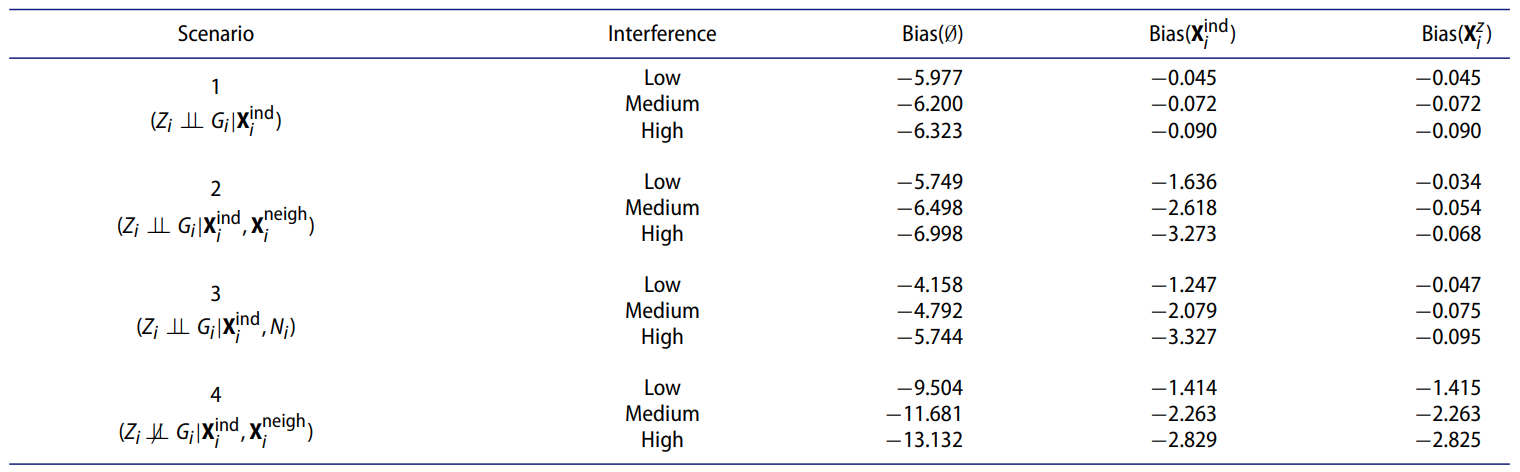
\includegraphics[scale=0.45]{table1.png}
   \caption{Computed bias for $\tau$}
   \label{tab:tab1}
   \end{table}
  \end{wideitemize}
 \end{column}%
\hfill%
\begin{column}{.38\textwidth}
  %
  \vspace{20pt}
  %
  \vspace{20pt}
\end{column}%
\end{columns}
\end{frame}



\begin{frame}{Main Effects : Bias of Naive Estimators and GPS-Based Estimator}
\begin{columns}[T] % align columns
\begin{column}{\textwidth}
  \begin{wideitemize}
  \item  Table 2 reports the mean bias and root mean squared error of six estimators in all scenarios.  
   \begin{table}[h]
   \centering
   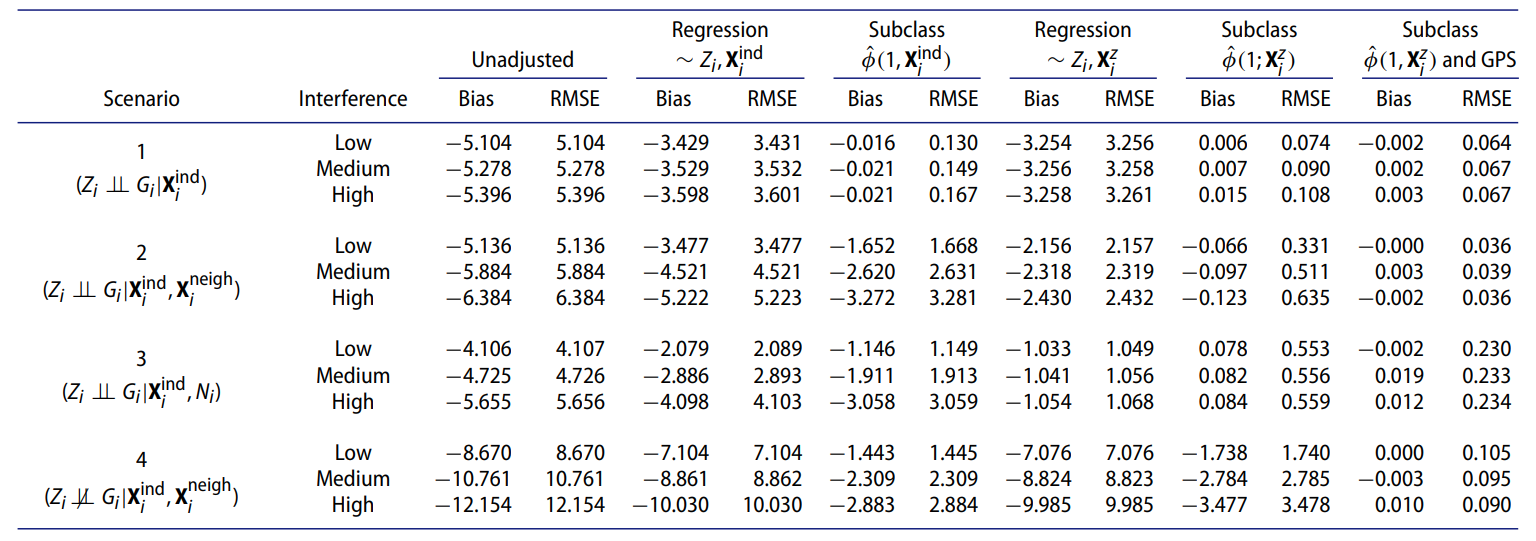
\includegraphics[scale=0.45]{table2.png}
   \caption{Estimation of main effect $\tau$}
   \label{tab:tab2}
   \end{table}
  \end{wideitemize}
\end{column}%
\hfill%
\begin{column}{.38\textwidth}
  %
  \vspace{20pt}
  %
  \vspace{20pt}
\end{column}%
\end{columns}
\end{frame}



\begin{frame}{Spillover Effects}
\begin{columns}[T] % align columns
\begin{column}{\textwidth}
  \begin{wideitemize}
  \item  Table 3 and Table 4 report the mean bias and root mean squared error of all estimators for spillover effects $\Delta(0)$ and $\Delta(1)$.  
   \begin{table}[h]
   \centering
   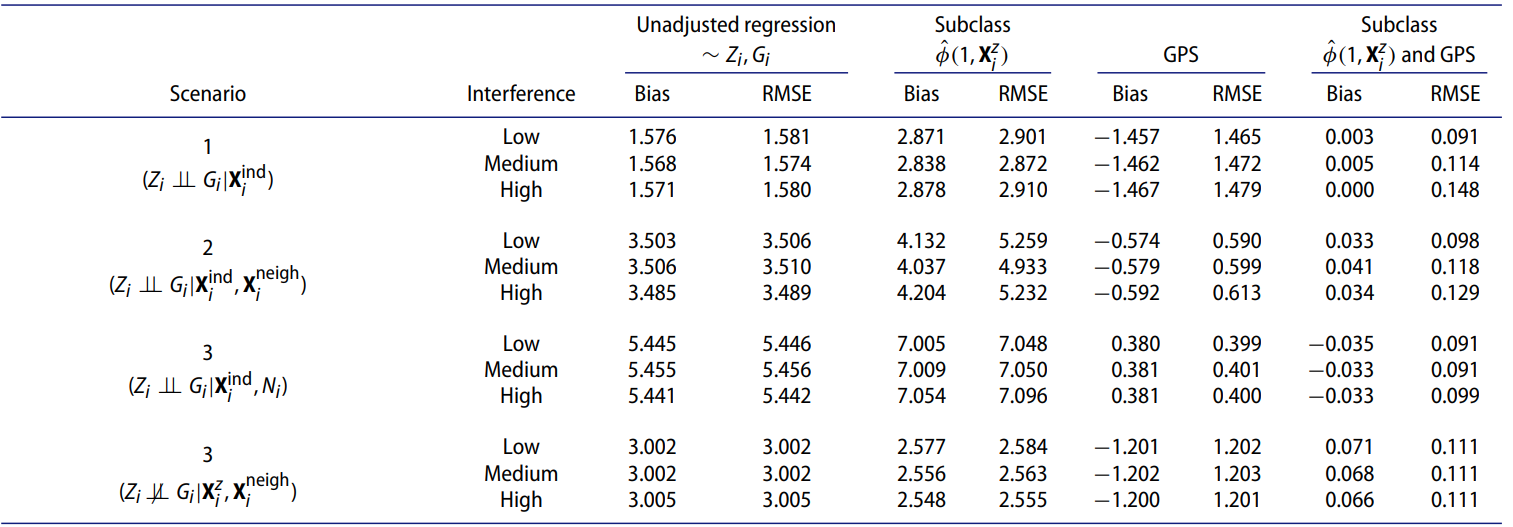
\includegraphics[scale=0.45]{table3.png}
   \caption{Estimation of  $\Delta(0)$}
   \label{tab:tab3}
   \end{table}
  \end{wideitemize}
\end{column}%
\hfill%
\begin{column}{.38\textwidth}
  %
  \vspace{20pt}
  %
  \vspace{20pt}
\end{column}%
\end{columns}
\end{frame}


\begin{frame}{Spillover Effects}
\begin{columns}[T] % align columns
\begin{column}{\textwidth}
  \begin{wideitemize}
   \begin{table}[h]
   \centering
   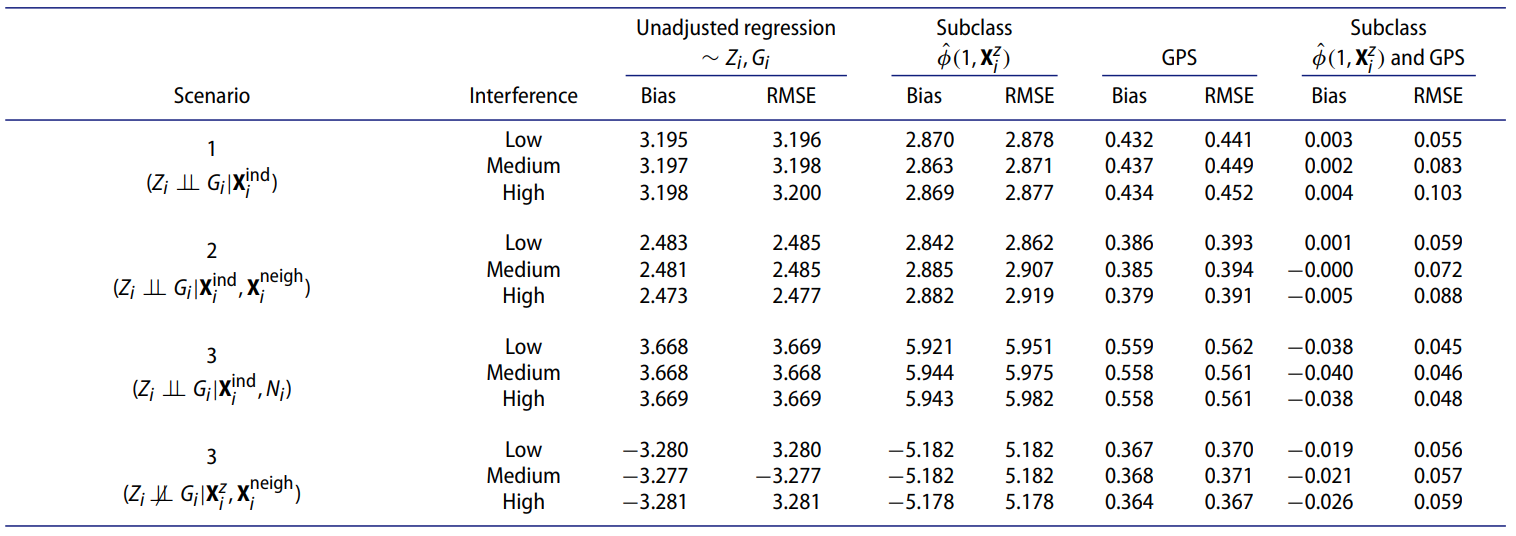
\includegraphics[scale=0.45]{table4.png}
   \caption{Estimation of  $\Delta(1)$}
   \label{tab:tab4}
   \end{table}
  \end{wideitemize}
\end{column}%
\hfill%
\begin{column}{.38\textwidth}
  %
  \vspace{20pt}
  %
  \vspace{20pt}
\end{column}%
\end{columns}
\end{frame}

\begin{frame}{Spillover Effects}
\begin{columns}[T] % align columns
\begin{column}{\textwidth}
  \begin{wideitemize}
  \item Figure 2 depicts the scatterplot of the observed outcomes and the estimated ADRFs $\mu(0,g)$ and $\mu(1,g)$ , $g \in \{0,0.2,0.4,0.6,0.8,1\}$ ,for Scenario 2
   \begin{figure}[h]
   \centering
   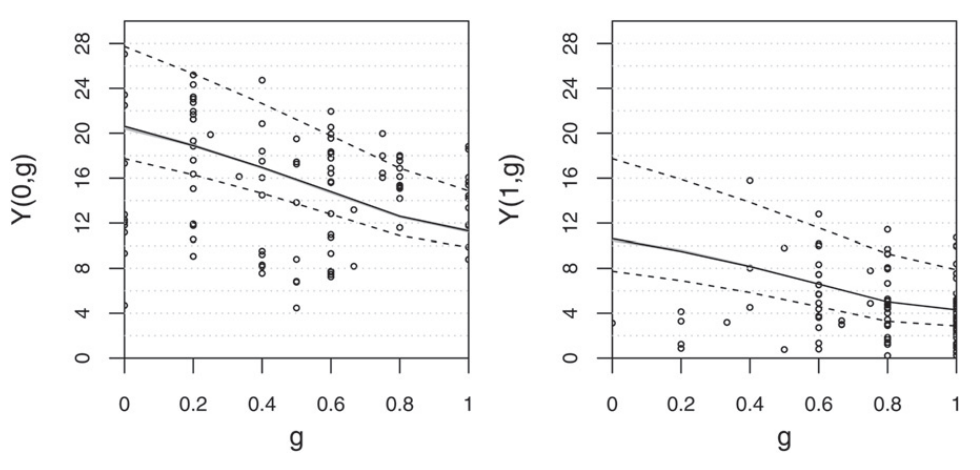
\includegraphics[scale=0.6]{figure2.png}
   \caption{Estimated dose-response function $\mu(0,g)$ and $\mu(1,g)$}
   \label{fig:fig2}
   \end{figure}
  \end{wideitemize}
\end{column}%
\hfill%
\begin{column}{.38\textwidth}
  %
  \vspace{20pt}
  %
  \vspace{20pt}
\end{column}%
\end{columns}
\end{frame}

\begin{frame}{Spillover Effects}
\begin{columns}[T] % align columns
\begin{column}{\textwidth}
  \begin{wideitemize}
  \item  Figure 3 depicts spillover effects $\delta(0,g)$  i.e $\mu(0,g)-\mu(0,0)$ and spillover effects $\delta(1,g)$ i.e $\mu(1,g)-\mu(1,0)$ 
   \begin{figure}[h]
   \centering
   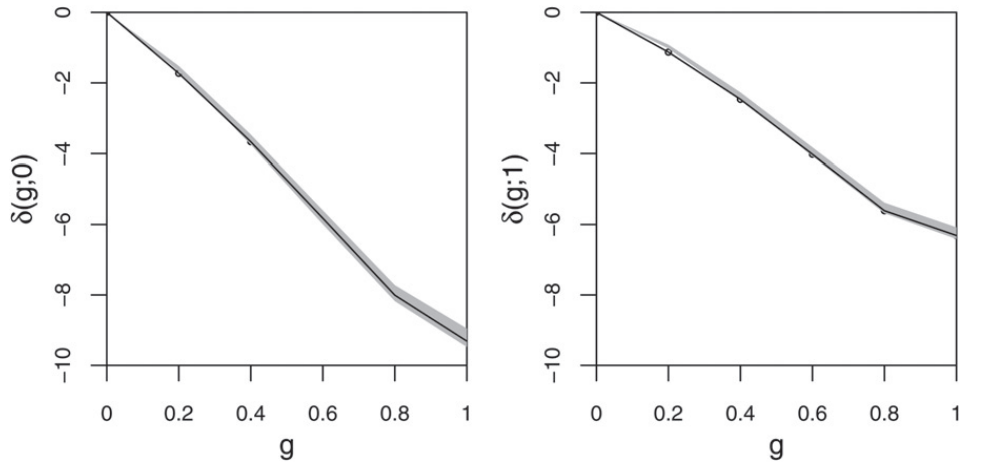
\includegraphics[scale=0.6]{figure3.png}
   \caption{Estimated spillover effects $\delta(g;z)$}
   \label{fig:fig3}
   \end{figure}
  \end{wideitemize}
\end{column}%
\hfill%
\begin{column}{.38\textwidth}
  %
  \vspace{20pt}
  %
  \vspace{20pt}
\end{column}%
\end{columns}
\end{frame}

\begin{frame}{Spillover Effects}
\begin{columns}[T] % align columns
\begin{column}{\textwidth}
  \begin{wideitemize}
  \item  Figure 4 depicts estimated main effects $\tau(g)$ . i.e $\mu(1,g)-\mu(0,g)$ .  
   \begin{figure}[h]
   \centering
   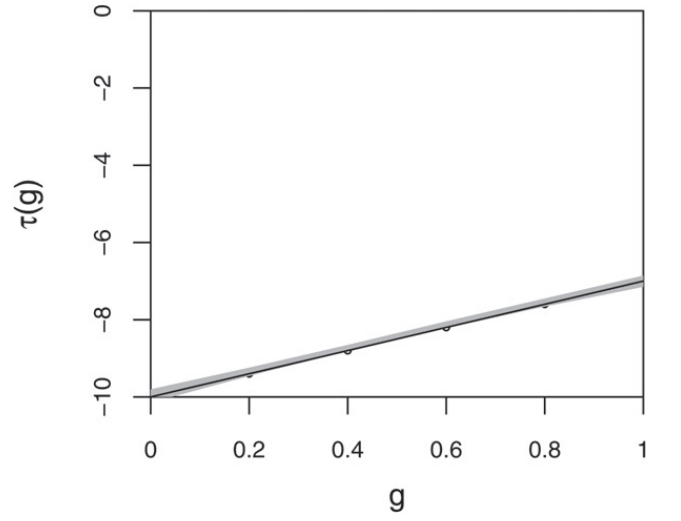
\includegraphics[scale=0.58]{figure4.png}
   \caption{Estimated main effects $\tau(g)$}
   \label{fig:fig4}
   \end{figure}
  \end{wideitemize}
\end{column}%
\hfill%
\begin{column}{.38\textwidth}
  %
  \vspace{20pt}
  %
  \vspace{20pt}
\end{column}%
\end{columns}
\end{frame}


\section{Conclusion}
\begin{transitionframe}
  \begin{center}
    { \Huge \textcolor{blue}{V . Conclusion}}
  \end{center}
\end{transitionframe}





\begin{frame}{Concluding Remarks}
\begin{columns}[T] % align columns
\begin{column}{\textwidth}
  \begin{wideitemize}
  \item  SUTVA $\longrightarrow$ SUTNVA , potential outcome $Y_i(\mathbf{Z}_i,\mathbf{G}_i)$
  \item simple assignment mechanism $\longrightarrow$ compound assignment mechanism 
  \item naive estimator $\longrightarrow$ Subclassfication and GPS estimator
  \item Bias sources : $\mathbf{Z}_{\mathcal{N}_i}$, $P(Z_{i,res},G_{i,res}|\mathbf{X}_i^{\star})$
  \item limitations : network fully known and fixed , model dependent 
  \item future : sensitivity analysis , Bayesian semi-parametric approaches , account for network uncertainty

  \end{wideitemize}
\end{column}%
\hfill%
\begin{column}{.38\textwidth}
  %
  \vspace{20pt}
  %
  \vspace{20pt}
\end{column}%
\end{columns}
\end{frame}



\begin{frame}{Software}
\begin{columns}[T] % align columns
\begin{column}{.8\textwidth}
  \begin{wideitemize}
      \item \href{https://nbviewer.org/github/mpleung/networkinference/blob/main/docs/tutorial/tutorial.ipynb}{\textcolor{blue}{networkinference}} - Python package by Michael P. Leung 
      \item \href{https://github.com/freshtaste/CausalModel}{\textcolor{blue}{CausalModel}} - Python package by Qu, Zhaonan and Xiong, Ruoxuan and Liu, Jizhou and Imbens, Guido 
      \item \href{https://cran.r-project.org/web/packages/inferference/index.html}{\textcolor{blue}{inferference}} - R package by Bradley Saul
      \item \href{https://cran.r-project.org/web/packages/clusteredinterference/index.html}{\textcolor{blue}{clusteredinterference}} - R package by Brian G. Barkley 
      \item \href{https://github.com/gpapadog/Interference}{\textcolor{blue}{Interference}} - R package by Georgia Papadogeorgou
  \end{wideitemize}
\end{column}
\end{columns}
\end{frame}


\begin{frame}
  \begin{center}
    { \Huge \textcolor{blue}{Thank You !}}
  \end{center}
\end{frame}


\end{document}


